\chapter{MÔ HÌNH BÀI TOÁN}

Trong chương này, chúng tôi trình bày các dạng toán học phục vụ cho việc mô tả một bài toán quy hoạch tuyến tính, bao gồm: dạng chuẩn, và dạng tăng cường. Với các dạng mô hình, chúng tôi trình bày các một số ví dụ minh họa tương ứng. Hơn nữa, chúng tôi cũng điểm qua tính đối ngẫu của bài toán LP.

\section{Dạng chuẩn LP}

Bài toán quy hoạch tuyến tính là bài toán tối ưu hóa mà bao gồm ba thành phần chính
\begin{itemize}
    \item Cực đại hóa (hoặc cực tiểu hóa) một hàm mục tiêu tuyến tính (hoặc hàm affine).
    \item Hàm mục tiêu có $n$ biến quyết định.
    \item Thỏa mãn một tập các ràng buộc mà được khai triển bởi các đẳng thức hoặc bất đẳng tuyến tính.
\end{itemize}

Dạng chuẩn của một bài toán LP như sau:
\begin{equation}
    \begin{aligned}
        \text{maximize/ minimize } \quad & c_1 x_1 + \dots + c_n x_n \\
        \text{subject to }\quad &
            \begin{array}{c}
            a_{11} x_1 + \dots + a_{1n} x_n = b_1 \\
            a_{21} x_1 + \dots + a_{2n} x_n = b_2 \\
            \vdots \\
            a_{m1} x_1 + \dots + a_{mn} x_n = b_m 
            \end{array} \\ 
            & x_1, x_2, ..., x_n \geq 0
    \end{aligned}   
\end{equation}
Trong đó: $b_i$, $c_i$ và $a_{ij}$ là các hằng số cố định, và $x_i$ là các biến số thực cần được quyết định. Giả định rằng mỗi phương trình đã được nhân với trừ đơn vị, thế nên $b_i \geq 0$

Trong dạng sử dụng ma trận, bài toán dạng chuẩn có thể viết một cách gọn hơn như sau:
\begin{equation}
    \begin{aligned}
    \text{maximize/ minimize } \quad & \mathbf{c}^{\top}\mathbf{x} & \\ 
    \text{subject to }\quad & \mathbf{Ax} = \mathbf{b} \\
    \quad& \mathbf{x} \geq \mathbf{0}\\
    \end{aligned}
\end{equation}
Trong đó: vector quyết định $\mathbf{x} \in \mathbb{R}^n$, vector hệ số dữ liệu mục tiêu $\mathbf{c}^{\top} \in \mathbb{R}^n$ , ma trận dữ liệu ràng buộc $\mathbf{A} \in \mathbb{R}^{m \times n}$, và vector dữ liệu bên phải $\mathbf{b} \in \mathbb{R}^{m}$. Ràng buộc bất đẳng thức $\mathbf{x} \geq \mathbf{0}$ ám chỉ mỗi thành phần của vector $\mathbf{x}$ là không âm.

% Về mặt bản chất, quy hoạch tuyến tính giải quyết vấn đề hệ bất phương trình tuyến tính. 
\section{Các dạng biến thể của LP}

Trong thực tế, các bài toán có thể được mô hình hóa thành những dạng khác nhau. Chúng tôi điểm qua những biến thể của quy hoạch tuyến tính mà có thể chuyển đổi về thành dạng chuẩn, bao gồm: dạng biến chùng, biến thừa, và biến tự do.

\subsection{Dạng biến chùng}

Ta xem xét bài toán LP trong trường hợp tập ràng buộc là các bất đẳng thức tuyến tính như sau:
\begin{equation}
    \label{eq:slack_var}
    \begin{aligned}
        \text{maximize/ minimize } \quad & c_1 x_1 + \dots + c_n x_n \\
        \text{subject to }\quad &
            \begin{array}{c}
            a_{11} x_1 + \dots + a_{1n} x_n \leq b_1 \\
            a_{21} x_1 + \dots + a_{2n} x_n \leq b_2 \\
            \vdots \\
            a_{m1} x_1 + \dots + a_{mn} x_n \leq b_m 
            \end{array} \\ 
            \quad & x_1, x_2, ..., x_n \geq 0 \\
    \end{aligned}   
\end{equation}

Bằng cách thêm vào bài toán các biến không âm $x_{n+i}, i=1...m$ để chuyển tập ràng buộc bất đẳng thức thành tập ràng buộc đẳng thức. Các biến này được gọi là các biến chùng:
\begin{equation}
    \label{eq:slack_var1}
    \begin{aligned}
        \text{maximize/ minimize } \quad & c_1 x_1 + \dots + c_n x_n \\
        \text{subject to }\quad &
            \begin{array}{c}
            a_{11} x_1 + \dots + a_{1n} x_n + x_{n+1} = b_1 \\
            a_{21} x_1 + \dots + a_{2n} x_n + x_{n+2}= b_2 \\
            \vdots \\
            a_{m1} x_1 + \dots + a_{mn} x_n + x_{n+m} = b_m 
            \end{array} \\ 
            \quad & x_1, x_2, ..., x_n,  x_{n+1}, ..., x_{n+m}\geq 0 \\
    \end{aligned}   
\end{equation}

\subsection{Dạng biến thừa}

Nếu ta đổi dấu các bất đẳng thức ràng buộc ở bài toán \ref{eq:slack_var}, ta được:
\begin{equation}
    \label{eq:surplus_var}
    \begin{aligned}
        \text{maximize/ minimize } \quad & c_1 x_1 + \dots + c_n x_n \\
        \text{subject to }\quad &
            \begin{array}{c}
            a_{11} x_1 + \dots + a_{1n} x_n \geq b_1 \\
            a_{21} x_1 + \dots + a_{2n} x_n \geq b_2 \\
            \vdots \\
            a_{m1} x_1 + \dots + a_{mn} x_n \geq b_m 
            \end{array} \\ 
            & x_1, x_2, ..., x_n \geq 0
    \end{aligned}   
\end{equation}

Xem xét một bất đẳng thức cụ thể thứ $i$
\begin{equation}
    a_{i1} x_1 + \dots + a_{in} x_n \geq b_i
\end{equation}

Dễ dàng biến đổi bất đẳng thức trên thành đẳng thức bằng cách:
\begin{equation}
    a_{i1} x_1 + \dots + a_{in} x_n - y_i = b_i
\end{equation}

Từ đó, ta dễ dàng chuyển đổi về dạng chuẩn LP. Những biến $y_i$ được gọi là biến thừa.

\subsection{Dạng biến tự do}

Nếu một bài toán LP cho trước ở dạng chuẩn mà có một hay nhiều biến ẩn không có ràng buộc dương, thì bài toán có thể được biến đổi về dạng chuẩn bằng một trong hai cách.
\begin{itemize}
    \item Cách 1: Biến đổi biến tự do dựa trên ràng buộc và thay thế vào hàm mục tiêu và các ràng buộc còn lại.
    \item Cách 2: Thêm biến vào bài toán.
\end{itemize}

\subsection{Ví dụ cụ thể}

Xem xét bài toán:
\begin{equation}
    \label{eq:ex1}
    \begin{aligned}
        \text{minimize } \quad & x_1 + 2x_2 + 3x_3 \\
        \text{subject to }\quad &
            \begin{array}{c}
            x_1 + x_2 + 2x_3 = 4 \\
            3x_1 + 4x_2 + 5x_3 = 9 \\
            \end{array} \\ 
            & x_2, x_3 \geq 0
    \end{aligned}   
\end{equation}

Bởi vì $x_1$ là biến tự do, dựa vào ràng buộc thứ nhất, ta có:

\begin{equation}
    x_1 = 4 - x_2 - 2x_3
\end{equation}

Thay vào hàm mục tiêu và ràng buộc thứ hai, ta thu được bài toán tương đương như sau:
\begin{equation}
    \label{eq:ex2}
    \begin{aligned}
        \text{minimize } \quad & 4 + x_2 + x_3 \\
        \text{subject to }\quad &
            \begin{array}{c}
            - x_2 + x_3 = 3 \\
            \end{array} \\ 
            & x_2, x_3 \geq 0
    \end{aligned}   
\end{equation}

\section{Tính đối ngẫu}

Mọi bài toán quy hoạch tuyến tính, được xem như bài toán gốc (primal), có thể được biến đổi thành một bài toán đối ngẫu mà cho ta một chặn trên đối với giá trị tối ưu của bài toán gốc. Nếu xem xét dạng ma trận, ta có thể khai triển bài toán primal như sau:



% \section{Lý thuyết về nghiệm tối ưu và cạnh tối ưu của đa diện}


\section{Các ví dụ thực tế về bài toán LP}

LP được xem như một mô hình hiệu quả trong việc giải quyết nhiều bài toán thực tế liên quan đến các hiện tượng phân chia công việc và kinh tế học. 

\subsection{Bài toán ăn kiêng - Diet Problem}

Làm thế nào chúng ta có thể xác định được chế độ ăn uống tiết kiệm nhất, đáp ứng được các yêu cầu dinh dưỡng tối thiểu cơ bản để có sức khỏe tốt? Đó là một bài toán khó, nhất là với một chuyên gia dinh dưỡng trong quân đội. Và thật vậy, bài toán này là một trong những bài toán tối ưu hóa đầu tiên được nghiên cứu vào những năm 1930 và 1940. Vấn đề được thúc đẩy bởi mong muốn của Quân đội nhằm giảm thiểu chi phí cho lính GI ăn tại thực địa trong khi vẫn cung cấp chế độ ăn uống lành mạnh. Một trong những nhà nghiên cứu đầu tiên nghiên cứu vấn đề này là George Stigler, người đã đưa ra phỏng đoán có căn cứ về giải pháp tối ưu bằng phương pháp heuristic. Dự đoán của ông về chi phí cho một chế độ ăn tối ưu là 39,93 USD mỗi năm (giá năm 1939).

Để minh họa, chúng ta sẽ xem xét bài toán dưới góc độ đơn giản. Giả định rằng cho sẵn trong siêu thị $n$ thức ăn khác nhau, thức ăn thứ $j$ có mức giá $c_j$ trên một đơn vị. Ngoài ra còn có $m$ thành phần dinh dưỡng cơ bản và để đạt được một chế độ ăn lành mạnh (balance diet), mỗi cá nhân cần phải nhận được ít nhất $b_i$ đơn vị của thành phần dinh dưỡng thứ $i$ trên một ngày. Cuối cùng, giả định rằng mỗi đơn vị thức ăn chứa $a_{ij}$ đơn vị của thành phần dinh dưỡng thứ $i$. Ta có thể mô tả bài toán dưới dạng công thức như sau:

\begin{equation}
    \label{eq:diet_problem}
    \begin{aligned}
        \text{minimize } \quad & c_1x_1 + c_2x_2 + ... + c_nx_n\\
        \text{subject to }\quad &
            \begin{array}{c}
            a_{i1}x_1 + a_{i2}x_2 + ... + a_{in}x_n \geq b_i, i = 1...m \\
            \end{array} \\ 
            & x_1, x_2, ..., x_n \geq 0
    \end{aligned}   
\end{equation}

\subsection{Bài toán phân phối tài nguyên - Resource-Allocation Problem}

Giả sử chúng ta sở hữu một cơ sở có khả năng sản xuất $n$ sản phẩm khác nhau, mỗi sản phẩm có thể yêu cầu lượng $m$ tài nguyên khác nhau. Mỗi sản phẩm cần được sản xuất ở bất kỳ mức độ $x_j \geq 0, j = 1,..,n$ nào, và mỗi đơn vị của sản phẩm thứ $j$ có thể được bán với giá $\pi_j$ và cần có $a_{ij}$ đơn vị của tài nguyên thứ $i, i = 1, ..., m$. Giả định rằng việc sản xuất sản phẩm có tính tuyến tính, nếu cho trước một tập gồm $m$ số $b_1, b_2, ..., b_m$ thể hiện định lượng sẵn có của $m$ nguồn tài nguyên, và ta mong muốn việc sản xuất sản phẩm đạt doanh thu tối đa. Bài toán này là một bài toán quy hoạch tuyến tính:

\begin{equation}
    \label{eq:resource_allocation_problem}
    \begin{aligned}
        \text{minimize } \quad & \pi_1x_1 + \pi_2x_2 + ... + \pi_nx_n\\
        \text{subject to }\quad &
            \begin{array}{c}
            a_{i1}x_1 + a_{i2}x_2 + ... + a_{in}x_n \geq b_i, i = 1...m \\
            \end{array} \\ 
            & x_1, x_2, ..., x_n \geq 0
    \end{aligned}   
\end{equation}

\subsection{Bài toán vận chuyển - Transportation Problem}

Mục tiêu của bài toán vận chuyển là giảm thiểu chi phí vận chuyển của một mặt hàng nhất định từ nguồn hoặc nơi xuất xứ (ví dụ: nhà máy) đến điểm đích (ví dụ: kho hàng, khách hàng cuối cùng), thỏa mãn tất cả các ràng buộc được yêu cầu không chỉ bởi nơi xuất xứ (ví dụ: tối đa số lượng hàng hóa có thể được gửi từ đó) mà còn theo điểm đến (ví dụ: số lượng sản phẩm tối thiểu cần được vận chuyển đến kho, số lượng sản phẩm theo yêu cầu của mỗi khách hàng). Ngoài những ràng buộc này, cũng cần xem xét chi phí vận chuyển hàng hóa từ nơi đi đến nơi đến (chi phí vận chuyển).

\begin{figure}[h!]
    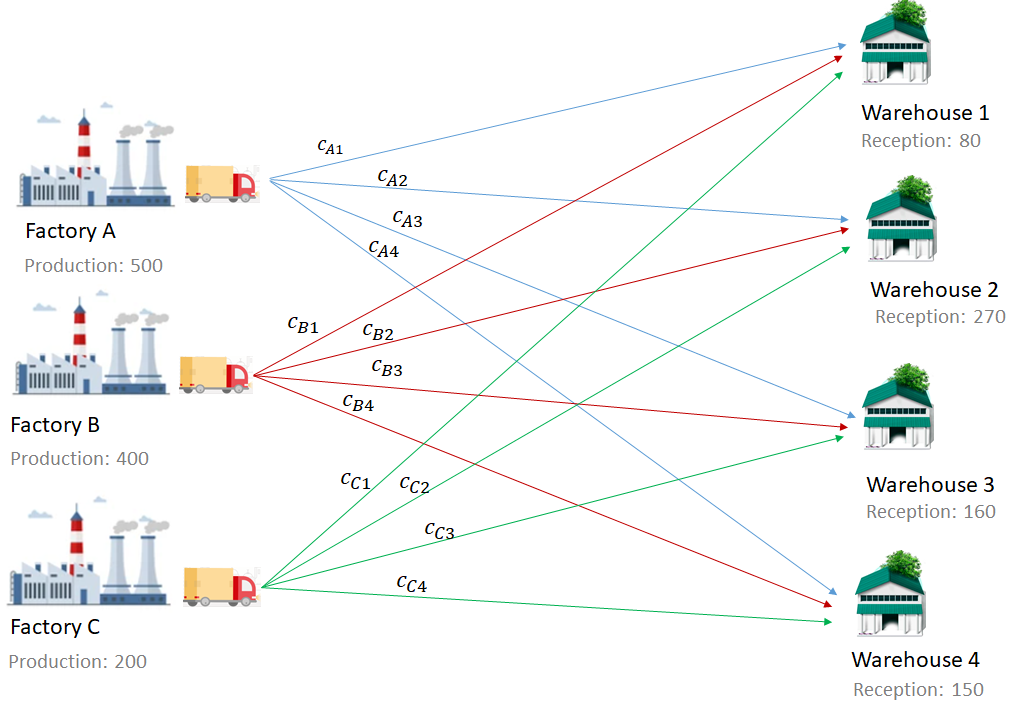
\includegraphics[width=0.85\linewidth]{figures/transport-problem.png}
    \caption{Minh họa về bài toán vận chuyển.}
    \label{fig:flow_network}
\end{figure}

Trước hết, gọi các định lượng $a_1, a_2, ..., a_m$ của một sản phẩm cụ thể cần được gửi đi từ mỗi một $m$ vị trí và nhận với số lượng $b_1, b_2, ..., b_n$ tương ứng tại mỗi $n$ điểm đích. Với mỗi việc giao sản phẩm, một đơn vị sản phẩm từ vị trí nguồn $i$ đến vị trí đích $j$ tiêu hao chi phí $c_{ij}$. Gọi $x_{ij}$ là số sản phẩm giao giữa mỗi cặp vị trí nguồn và đích, $i= 1...m$ và $j=1...n$; cần phải tìm $x_{ij}$ để thỏa mãn yêu cầu vận chuyển và cực tiểu tổng chi phí của công việc vận chuyển. Và ta có bài toán quy hoạch tuyến tính như sau:

\begin{equation}
    \label{eq:transport_problem}
    \begin{aligned}
        \text{minimize } \quad & \sum_{ij} c_{ij}x_{ij}\\
        \text{subject to }\quad & \sum_{j=1}^nx_{ij} = a_i, i = 1, ...m \\ 
        & \sum_{i=1}^mx_{ij} = b_j, j = 1, ...n \\ 
            & x_{ij} \geq 0, i = 1, ...m; j = 1, ...n
    \end{aligned}   
\end{equation}

\subsection{Bài toán luồng cực đại - Maximal Flow Problem}

Có một số bài toán thực tế có thể được mô hình hóa dưới dạng các luồng trong đồ thị đặc biệt gọi là luồng trên mạng. Luồng trên mạng là một đồ thị có hướng có các cạnh được dán nhãn bằng các số không âm biểu thị thông lượng của một loại dòng chảy nào đó: năng lượng điện, hàng hóa sản xuất sẽ được phân phối hoặc phân phối nước thành phố. Hình \ref{fig:flow_network} là một ví dụ trừu tượng về luồng trên mạng.

\begin{figure}[h!]
    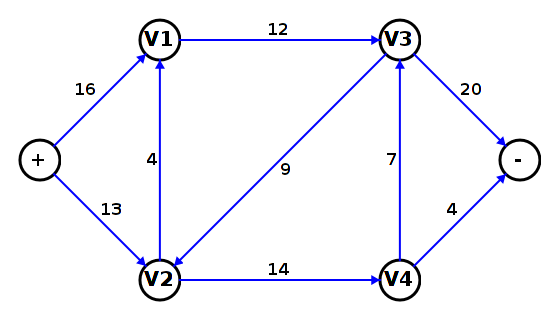
\includegraphics[width=0.85\linewidth]{figures/flow-network.png}
    \caption{Minh họa về một luồng trên mạng.}
    \label{fig:flow_network}
\end{figure}

Mạng luồng có thể có các đỉnh đặc biệt gọi là nguồn (sources) và đích (sinks).
\begin{itemize}
    \item Một nguồn tạo ra hoặc tạo ra bất cứ thứ gì đang chảy trong mạng. Đỉnh "+" thể hiện điểm nguồn trong luồng trên mạng trong Hình \ref{fig:flow_network}. Tùy thuộc vào bản chất chính xác của vấn đề, nguồn cũng có thể có giới hạn hoặc công suất.
    \item Một đích tiêu thụ bất cứ thứ gì đang chảy trong mạng. Đỉnh "-" thể hiện điểm đích trong luồng trên mạng trong Hình \ref{fig:flow_network}. Tùy thuộc vào bản chất chính xác của vấn đề, điểm đích cũng có thể có giới hạn hoặc dung tích.
\end{itemize}

Nút nguồn và nút đích của một mạng là phân biệt nhau, ta gọi chúng lần lượt là nút 1 và nút $m$. Tất cả các nút còn lại phải thỏa mãn điều kiện rằng lưu lượng vào chúng bằng 0. Tuy nhiên, nút nguồn có một luồng lưu lượng ra và nút đích có một luồng lưu lượng vào. Luồng lưu lượng ra $f$ của nút nguồn sẽ bằng luồng lưu lượng vào của nút đích như một hệ quả vì điều kiện của các nút còn lại. 

Một tập hợp các luồng cung thỏa mãn các điều kiện này được gọi là một luồng trong mạng có giá trị $f$. Bài toán luồng cực đại là vấn đề xác định luồng cực đại có thể được thiết lập trong mạng như vậy.

\begin{equation}
    \label{eq:transport_problem}
    \begin{aligned}
        \text{maximize } \quad & f\\
        \text{subject to }\quad & \sum_{j=1}^nx_{1j} - \sum_{j=1}^nx_{j1} - f = 0\\ 
        & \sum_{j=1}^nx_{ij} - \sum_{j=1}^nx_{ji} = 0, i \ne 1, m \\
        & \sum_{j=1}^nx_{mj} - \sum_{j=1}^nx_{jm} + f = 0 \\
            & 0 \leq x_{ij} \leq k_{ij}, \forall i, j
    \end{aligned}   
\end{equation}

\subsection{Bài toán chuỗi cung ứng - Supply-Chain Problem}

\subsection{Bài toán tối ưu phân lớp tuyến tính và Support Vector Machine}

\begin{figure}[h!]
    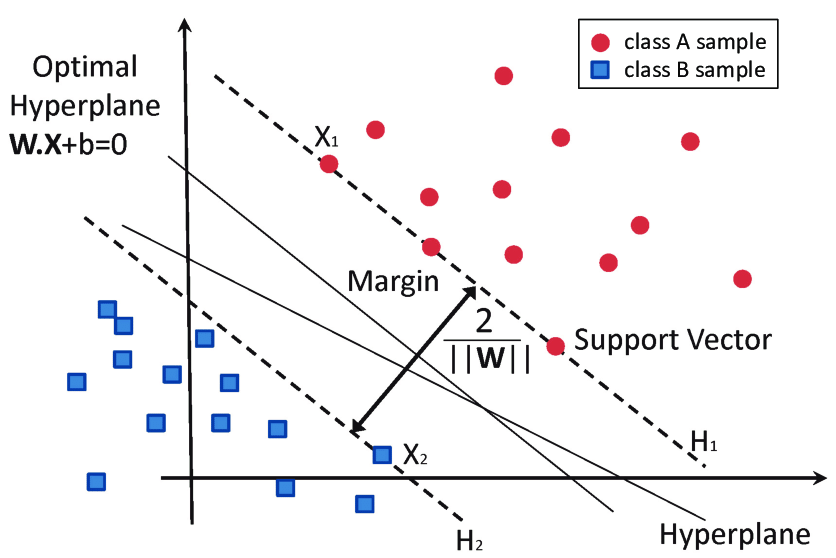
\includegraphics[width=0.85\linewidth]{figures/svm.png}
    \caption{Minh họa về support vector machine.}
    \label{fig:flow_network}
\end{figure}